\section{Performance and Analysis}
Scaletta:\\
- presentazione datatset (con grafici sulla distribuzione dei degree)\\
- risultati ottenuti (modularità e tempo) sull'intero dataset rispetto sequenziale\\
- analisi prima fase ottimizzazione dei due algoritmi e fast move\\
- analisi aggregazione\\
- algoritmo ibrido\\

\subsection{Datasets}
In this section we present the 13 dataset used in this thesis. These datasets coming from three main sources: the Stanford Stanford Large Network Dataset Collection (also known as SNAP) \cite{snap}, the Florida Sparse Matrix Collection \cite{florida-matrix} and the the Koblenz Network Collection (also known as KONECT)  \cite{konect}. In the Table \ref{tab:dataset} there are a briefly presentation of the dataset and in Figure \ref{fig:dataset-degree-distribution} there are the degree distribution of the graphs.  We point out that even if all this graph are unweighted, some of it are directed: during the parsing phase we doesn't keep the "directness" of the graph, and we treat it as a undirected one as required from the algorithm. In addition, if in the original graph there are some repeated edges, we consider it once. In the table \ref{tab:dataset} the number of edges are those obtained after this parsing, ordered by increasing edges number. Now we present the datasets:
\begin{table}
	\centering
	\begin{tabular}{ |l||c||r|r|}
		\hline
		\multicolumn{4}{|c|}{Datasets} \\
		\hline
		Name& Source &  Number of nodes  & Number of edges\\
		\hline
		coPapersDBLP & Florida  & 540.486    & 15.245.729\\
		patentCite & KONECT &3.774.768 & 16.518.947 \\
		packing-500x100x100-b050 & Florida & 2.145.839 & 17.488.243 \\
		soc-pokec-relationship & SNAP &1.632.803 & 22.301.964 \\ 
		delaunay\_n23 & Florida &8.388.608 & 25.165.784\\
		soc-LiveJournal1 & SNAP & 4.847.571 & 43.369.619 \\
		wikipedia\_link\_ja & KONECT & 1.610.638 & 56.237.763\\
		hollywood-2009 & Florida &1.139.905 & 57.515.616 \\
		wikipedia\_link\_it & KONECT & 1.865.965 & 68.049.979\\
		wikipedia\_link\_fr & KONECT & 3.023.165 & 83.472.152\\
		com-orkut & SNAP &3.072.441 &117.185.083\\
		wikipedia\_en(dbpedia) & KONECT & 18.268.991 & 126.890.209 \\
		indochina-2004 & Florida & 7.414.768 & 153.487.303 \\
		\hline
	\end{tabular}
	\caption{\label{tab:dataset}Datasets overview}
\end{table} 
\begin{itemize}
	\item \textbf{coPapersDBLP:} this graph model the citation and co-author network from the DBLP - Digital Bibliography and Library Project. Each node represent an author and each edge a citation.
	\item \textbf{patentCite:} This is the citation network of patents registered with the United States Patent and Trademark Office. Each node is a patent, and a directed edge represents a patent and an edge represents a citation. The network contain loops. This graph is also directed.
	\item \textbf{packing-500x100x100-b050:} this is a synthetic graph from numerical simulation.  
	\item \textbf{soc-pokec:} Pokec is the most popular on-line social network in Slovakia. Pokec has been provided for more than 10 years and connects more than 1.6 million people. This dataset map the relationship between people.
	\item \textbf{delaunay\_n23:} given a random set of point, in this graph represent a Delaunay triangulations of them.
	\item \textbf{soc-LiveJournal1}: LiveJournal is a free on-line community with almost 10 million members; a significant fraction of these members are highly active. LiveJournal allows members to maintain journals, individual and group blogs, and it allows people to declare which other members are their friends they belong. This graph model these friendship relations. 
	\item \textbf{wikipedia\_link\_jp:} This network consists of the wikilinks of the Wikipedia in the Japanese language (.ja). Nodes are Wikipedia articles, and directed edges are hyperlinks. Only pages in the article namespace are included. This graph is directed and some self-loop is possible.
	\item \textbf{hollywood-2009}: The graph of           
	movie actors. Vertices are actors, and two actors are joined             
	by an edge whenever they appeared in a movie together. The data date back to 2009. 
	\item \textbf{wikipedia\_link\_it:} This network consists of the wikilinks of the Wikipedia in the Italian language (it). Nodes are Wikipedia articles, and directed edges are hyperlinks. Only pages in the article namespace are included. This graph is directed and some self-loop is possible.
	\item \textbf{wikipedia\_link\_fr:} This network consists of the wikilinks of the Wikipedia in the French language (.fr). Nodes are Wikipedia articles, and directed edges are hyperlinks. Only pages in the article namespace are included. This graph is directed and some self-loop is possible.
	\item \textbf{com-orkut:} Orkut is a social-network where users form friendship each other: the nodes represent the users and the edges the friendship between them.
	\item \textbf{wikipedia\_en (dbpedia)}: The network is the hyperlink network of Wikipedia, as extracted in DBpedia. Nodes are pages in Wikipedia and edges correspond to hyperlinks (also known as wikilinks). The edges correspond to the relationships in DBpedia.
	Network info. The original graph is directed and multiple edges are possible.
	\item \textbf{indochina-2004}: A fairly large crawl of the country domains of Indochina performed for the Nagaoka University of Technology. This is a directed graph and each node represent a site and each edge a link from one site to another.
\end{itemize}

\begin{figure}
	\centering
	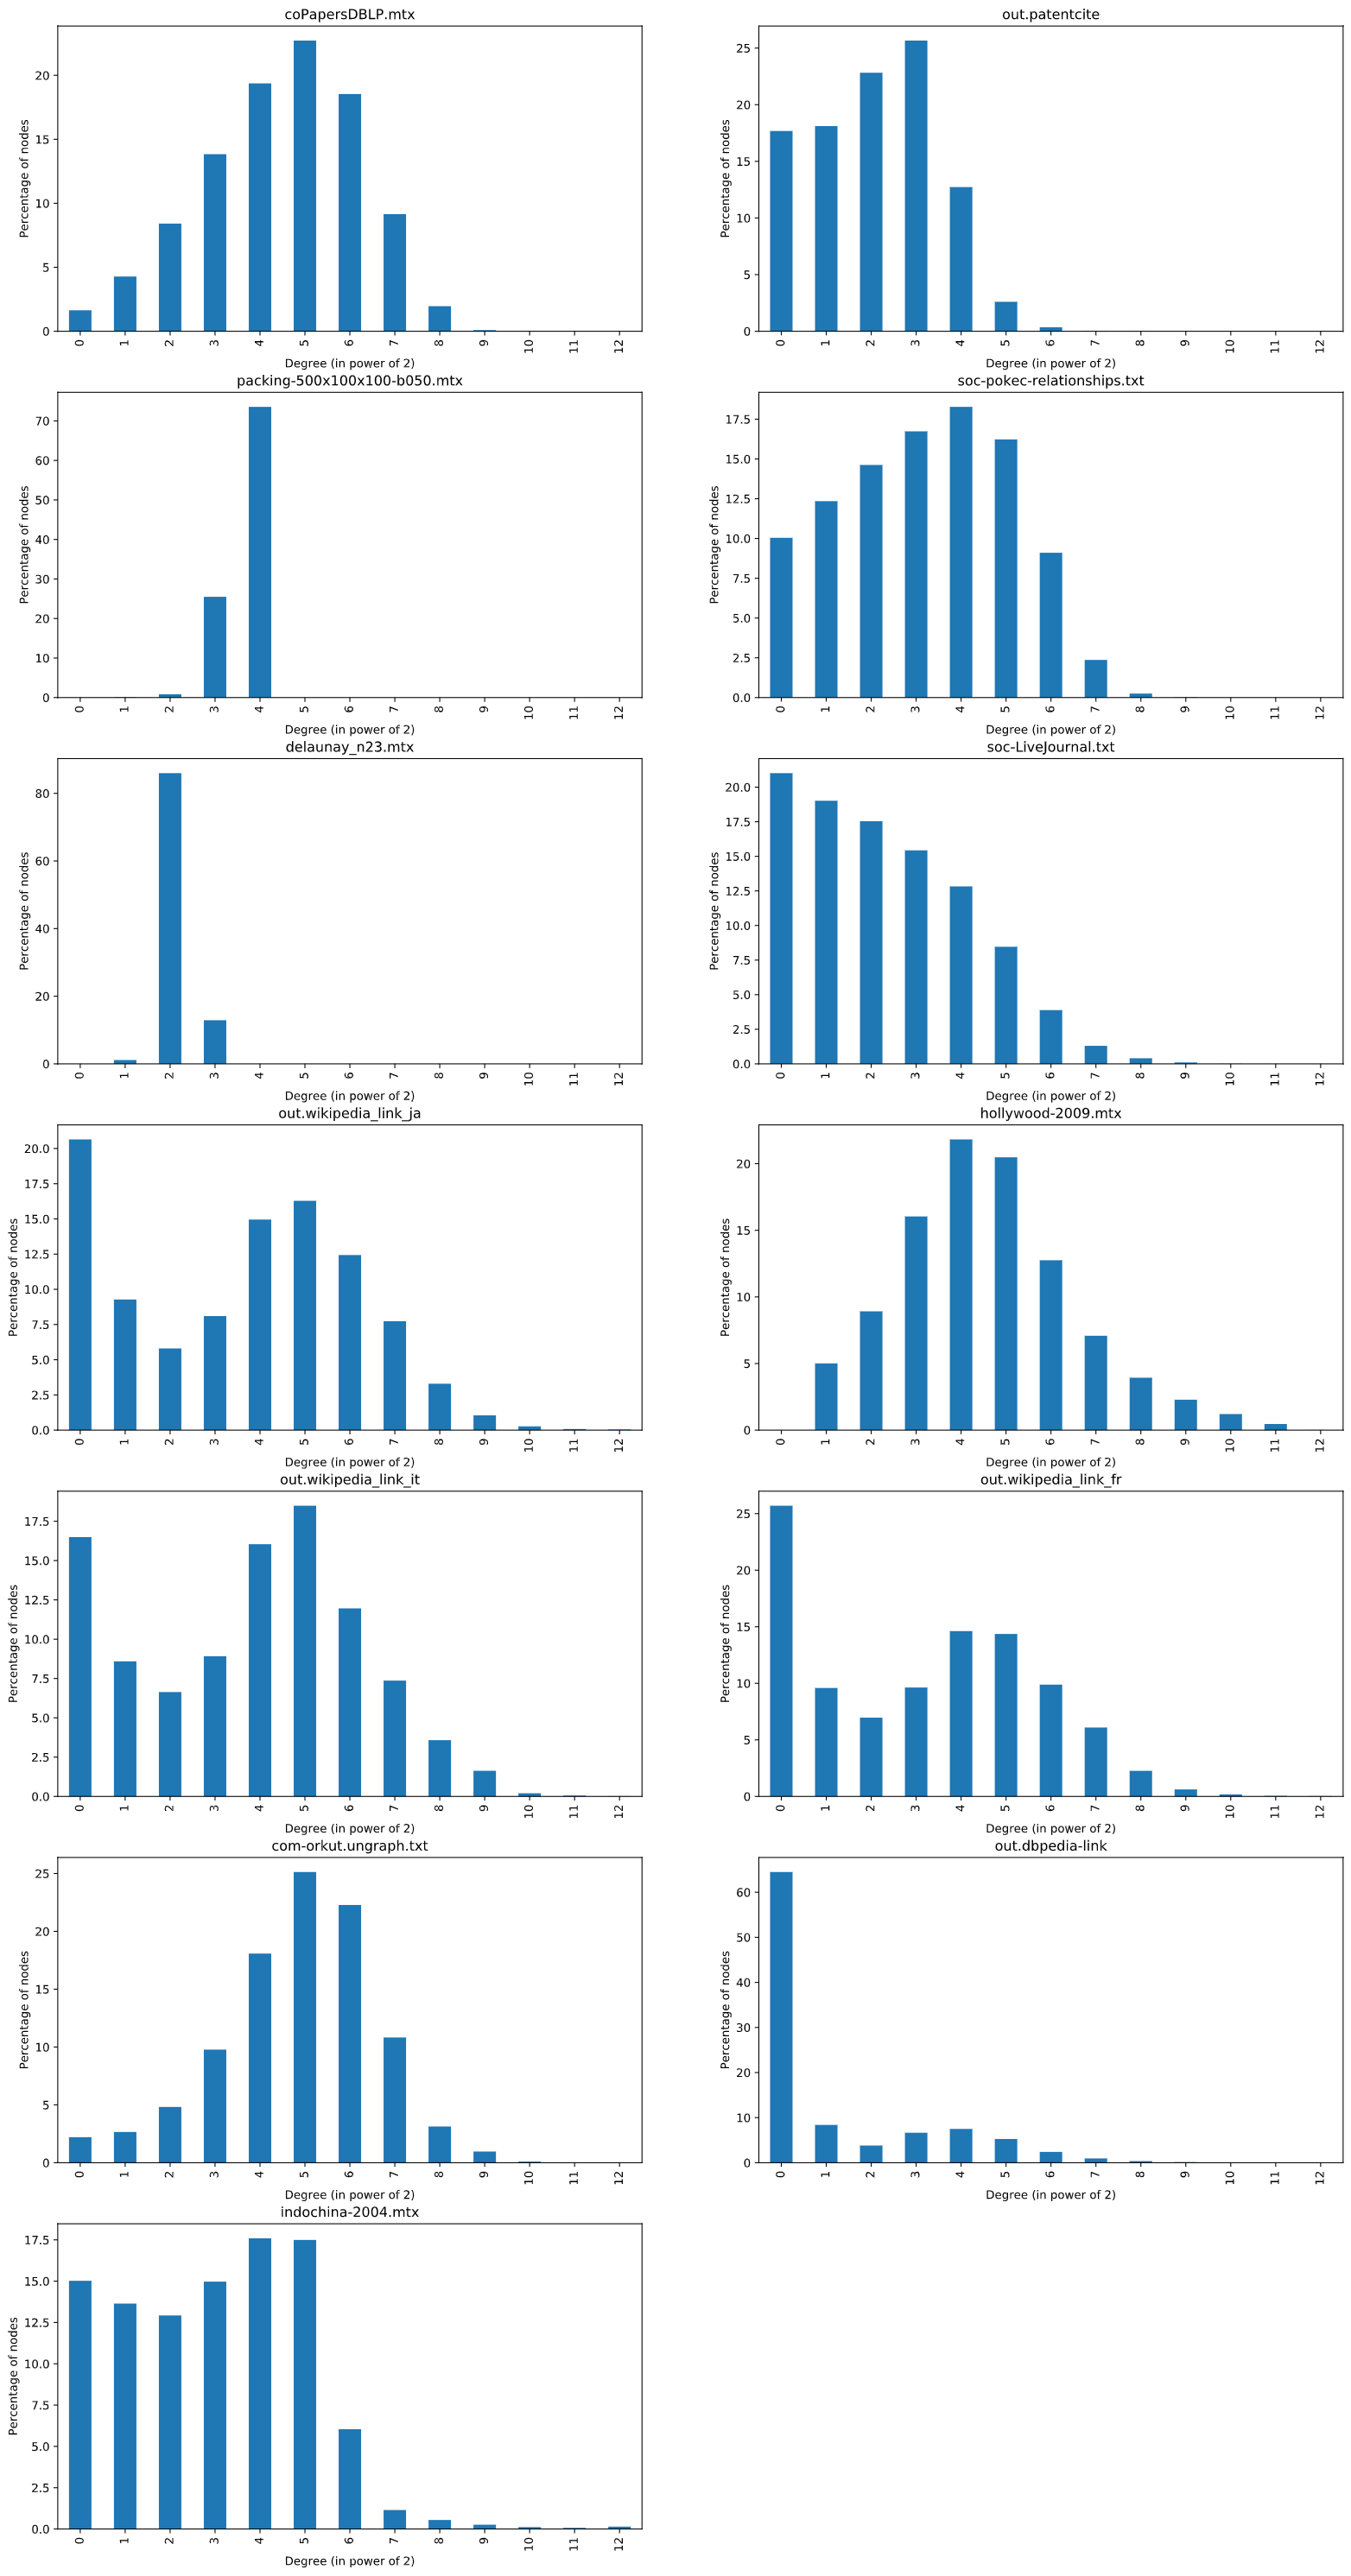
\includegraphics[width=0.75\linewidth]{0-resources/dataset-degree-distribution.png}
	\caption{Degree distribution in the datasets: we divide the nodes in ordered classes where in the class $i$ there are all the nodes with degree in range $[2^i, 2^{i+1})$. On the $x$-axes there are these classes; on the $y$ axes there is the percentage of nodes assigned to them.}
	\label{fig:dataset-degree-distribution}
\end{figure}
\newpage
\subsection{Results Overview}
In this section we present an overview of the obtained results and we make some general consideration about it. Some more insights about the first optimization phase and about the aggregation phase are presented next and we make some consideration in light of what we present in this section.\\ 
The algorithms was run on a Ubuntu 18.04.4 LTS machine with a 2.10GHz  Intel(R) Xeon(R) Silver 4110 CPU, a TITAN Xp GPU with 12 GB of memory and CUDA 10.2. To run our code we need a Nvidia GPU with a compute capability $\geq$ 3.5 due to the 64 bits \verb|atomicMax| operation used in the hash version. This GPU have a compute capability 6.1, so it comply with the technical specification.
We remark that we keep executing our optimization phase until the value of $\Delta Q$ between the various iteration is greater than a threshold $t$. Both our parallel version in the test uses $t = 0.01$.\\
\begin{table}[h]
	\centering
	\begin{tabular}{ |l||r||r|r|}
		\hline
		\multicolumn{4}{|c|}{Modularity Score} \\
		\hline
		Graph & Sequential & Prune-Sort-Reduce & Hashmap \\
		\hline
		coPapersDBLP 			& 0,8490 & 0,8544 & 0,8544 \\
		patentCite 				& 0,8095 & 0,7911 & 0,7878 \\
		packing-500x100x100-b050& 0,9353 & 0,9434 & 0,9416 \\
		soc-pokec-relationship	& 0,6837 & 0,6934 & 0,6852 \\ 
		delaunay\_n23 			& 0,9881 & 0,9856 & 0,9857 \\
		soc-LiveJournal1 		& 0,7251 & 0,7491 & 0,7482 \\
		wikipedia\_link\_ja 	& 0,5928 & 0,5690 & 0,5724 \\
		hollywood-2009 			& 0,7511 & 0,7542 & 0,7542 \\
		wikipedia\_link\_it 	& 0,7221 & 0,7190 & 0,7196 \\
		wikipedia\_link\_fr 	& 0,6777 & 0,6834 & 0,6871 \\
		com-orkut 				& 0,6545 & 0,6613 & 0,6629 \\
		wikipedia\_en(dbpedia) 	& 0,6629 & 0,6612 & 0,6618 \\
		indochina-2004 			& 0,9638 & 0,9632 & 0,9632 \\
		\hline
	\end{tabular}
	\caption{\label{tab:mod}Modularity result}
\end{table} \\
First of all, we analyze the modularity score obtained by the two algorithms respect to the sequential version as presented in \cite{Blondel_2008} to check the correctness of the our algorithm. In the Table \ref{tab:mod} are exposed the obtained results. We notice that both the score of the algorithm are in pair between them and also with the sequential version for all the graphs, and in some case we obtain also a better result in the parallel implementations respect to the sequential version. This  may be due to the parallel optimization, changing all the communities assigned to the vertices simultaneously, can avoid some local maxima.
\begin{table}
	\centering
	\begin{tabular}{ |l||r||r|r|}
		\hline
		\multicolumn{4}{|c|}{Execution Times} \\
		\hline
		Graph & Sequential & Prune-Sort-Reduce & Hashmap \\
		\hline
		coPapersDBLP 			&  11.906,89 &   419,59 &  412,79 \\
		patentCite 				&  88.620,13 & 1.796,88 & 2.555,14 \\
		packing-500x100x100-b050&  13.746,14 & 1.045,25 & 1.090,03 \\
		soc-pokec-relationship	&  30.162,70 & 1.843,95 & 2.186,81 \\ 
		delaunay\_n23 			&  44.392,42 & 1.020,23 & 1.319,22 \\
		soc-LiveJournal1 		&  77.225,64 & 2.187,45 & 2.677,51 \\
		wikipedia\_link\_ja 	&  76.816,01 & 2.654,88 & 2.305,11 \\
		hollywood-2009 			&  52.306,71 & 2.092,09 & 1.758,27 \\
		wikipedia\_link\_it 	&  82.599,92 & 3.875,04 & 2.732,99 \\
		wikipedia\_link\_fr 	& 115.977,81 & 3.910,95 & 3.273,91 \\
		com-orkut 				& 193.835,34 & 7.566,90 & 7.484,10 \\
		wikipedia\_en(dbpedia) 	& 300.431,38 & 5.287,65 & 6.464,03 \\
		indochina-2004 			& 113.195,87 & 2.899,50 & 2.303,52 \\
		\hline
	\end{tabular}
	\caption{\label{tab:execution_time}Execution Time in milliseconds}
\end{table} \\
In the Table \ref{tab:execution_time} there are the execution time of the two algorithms respect to the sequential version. We notice a big improvement in the performance for both the algorithm respect to the sequential version: we obtain a speed-up in range of a variable factor from 12 to 56 for our two algorithms. 

\subsection{Pruning analysis}
In this section, we analyze the effectiveness of the pruning approach: we focus our research on the first optimization phase. As we said previously, the first optimization phase is the most time-requiring phase, consuming about 80\% of the time \cite{wickramaarachchi2014fast}, so the pruning approach should increase the performance especially in this phase.
\begin{figure}[h]
	\centering
	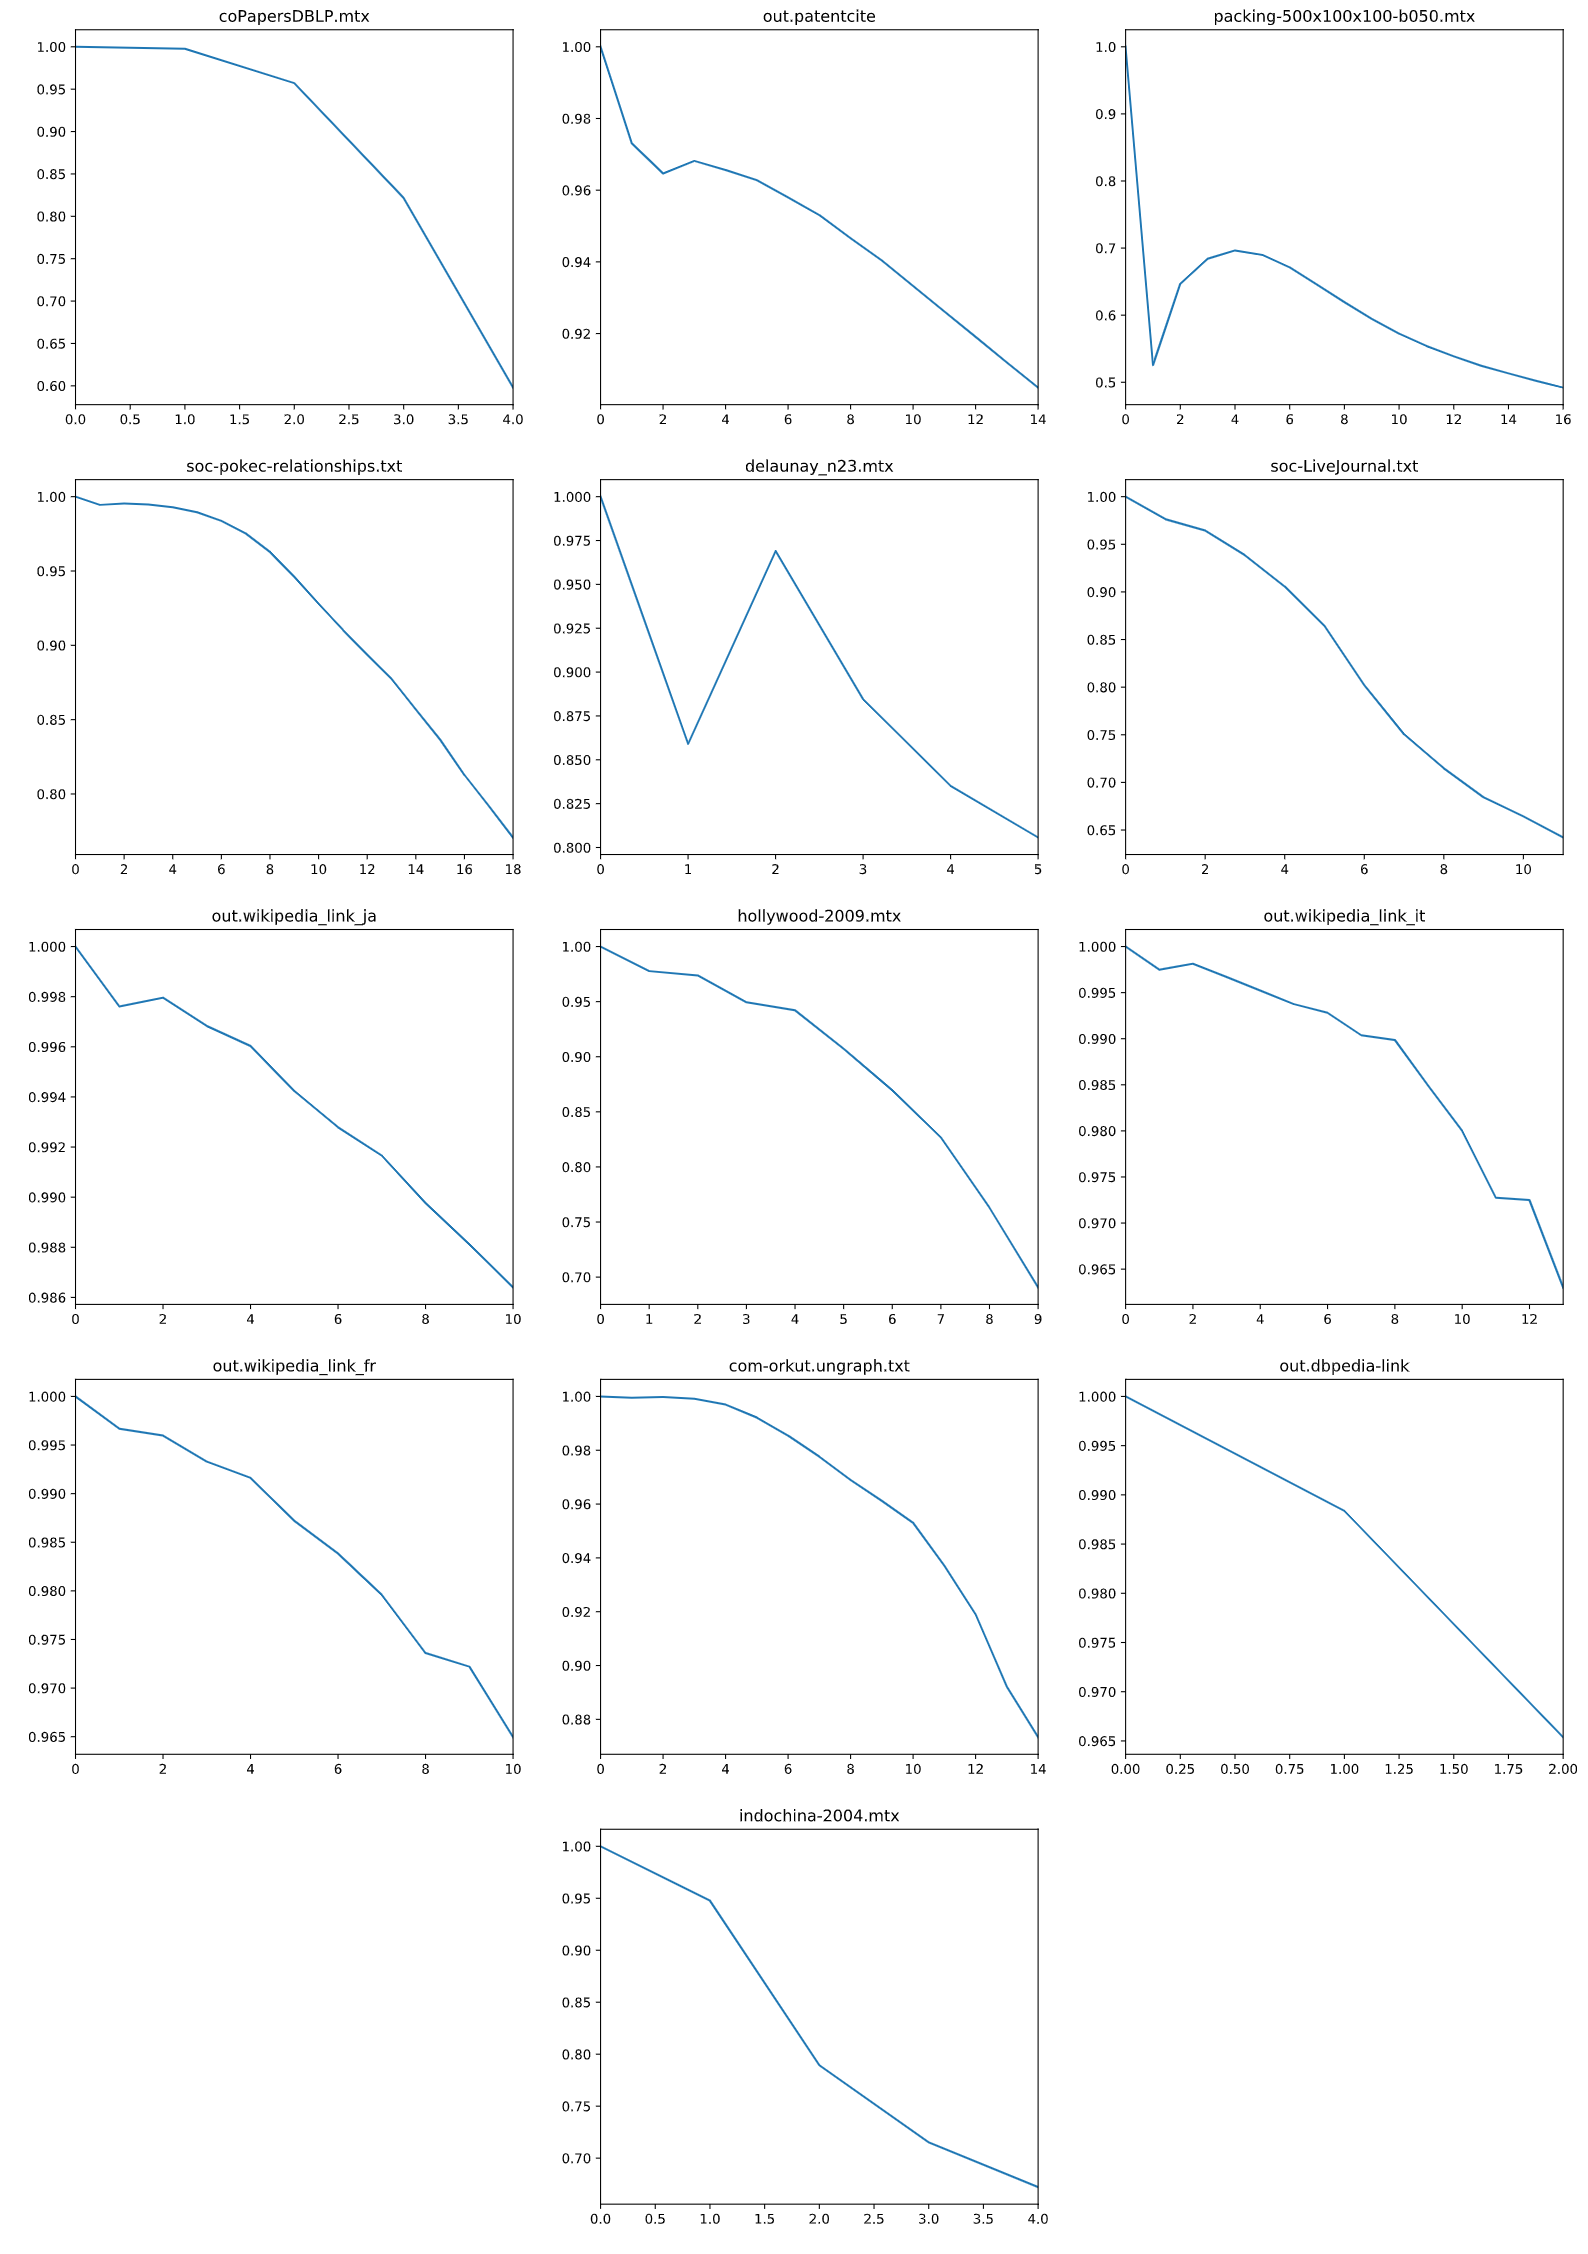
\includegraphics[width=0.7\linewidth]{0-resources/edge-percentage}
	\caption{Percentage of edge analyze in the first optimization phase}
	\label{fig:edge-percentage}
\end{figure}
We start from the Prune-Sort-Reduce version: first of all we present the percentage of the edges that we analyze in each iteration of the optimization phase (Figure \ref{fig:edge-percentage}). Exluding certain fluctuation at the earliest stage (we remark also that the two graph with the highest noise are two syntetic ones, i.e. packing-500x100x100-b050 and delaunay\_n23), we notice that the portion of the edges analyzed tend to decrease iteration by iteration. The percentage of reduction highly depends on the graph exterminated: we have the smallest reduction for the wikipedia\_link\_ja (only the $\sim\%2$ of the total are excluded in the last iteration); instead, in the graph packing-500x100x100-b050, we have run the optimization only on the $\sim\%50$ of the edges of the graph in last iteration. There are any direct correlation between the decrease of the number of the edges analyzed and the degree distribution of the nodes presented in Figure \ref{fig:dataset-degree-distribution}.
\begin{figure}[h]
	\centering
	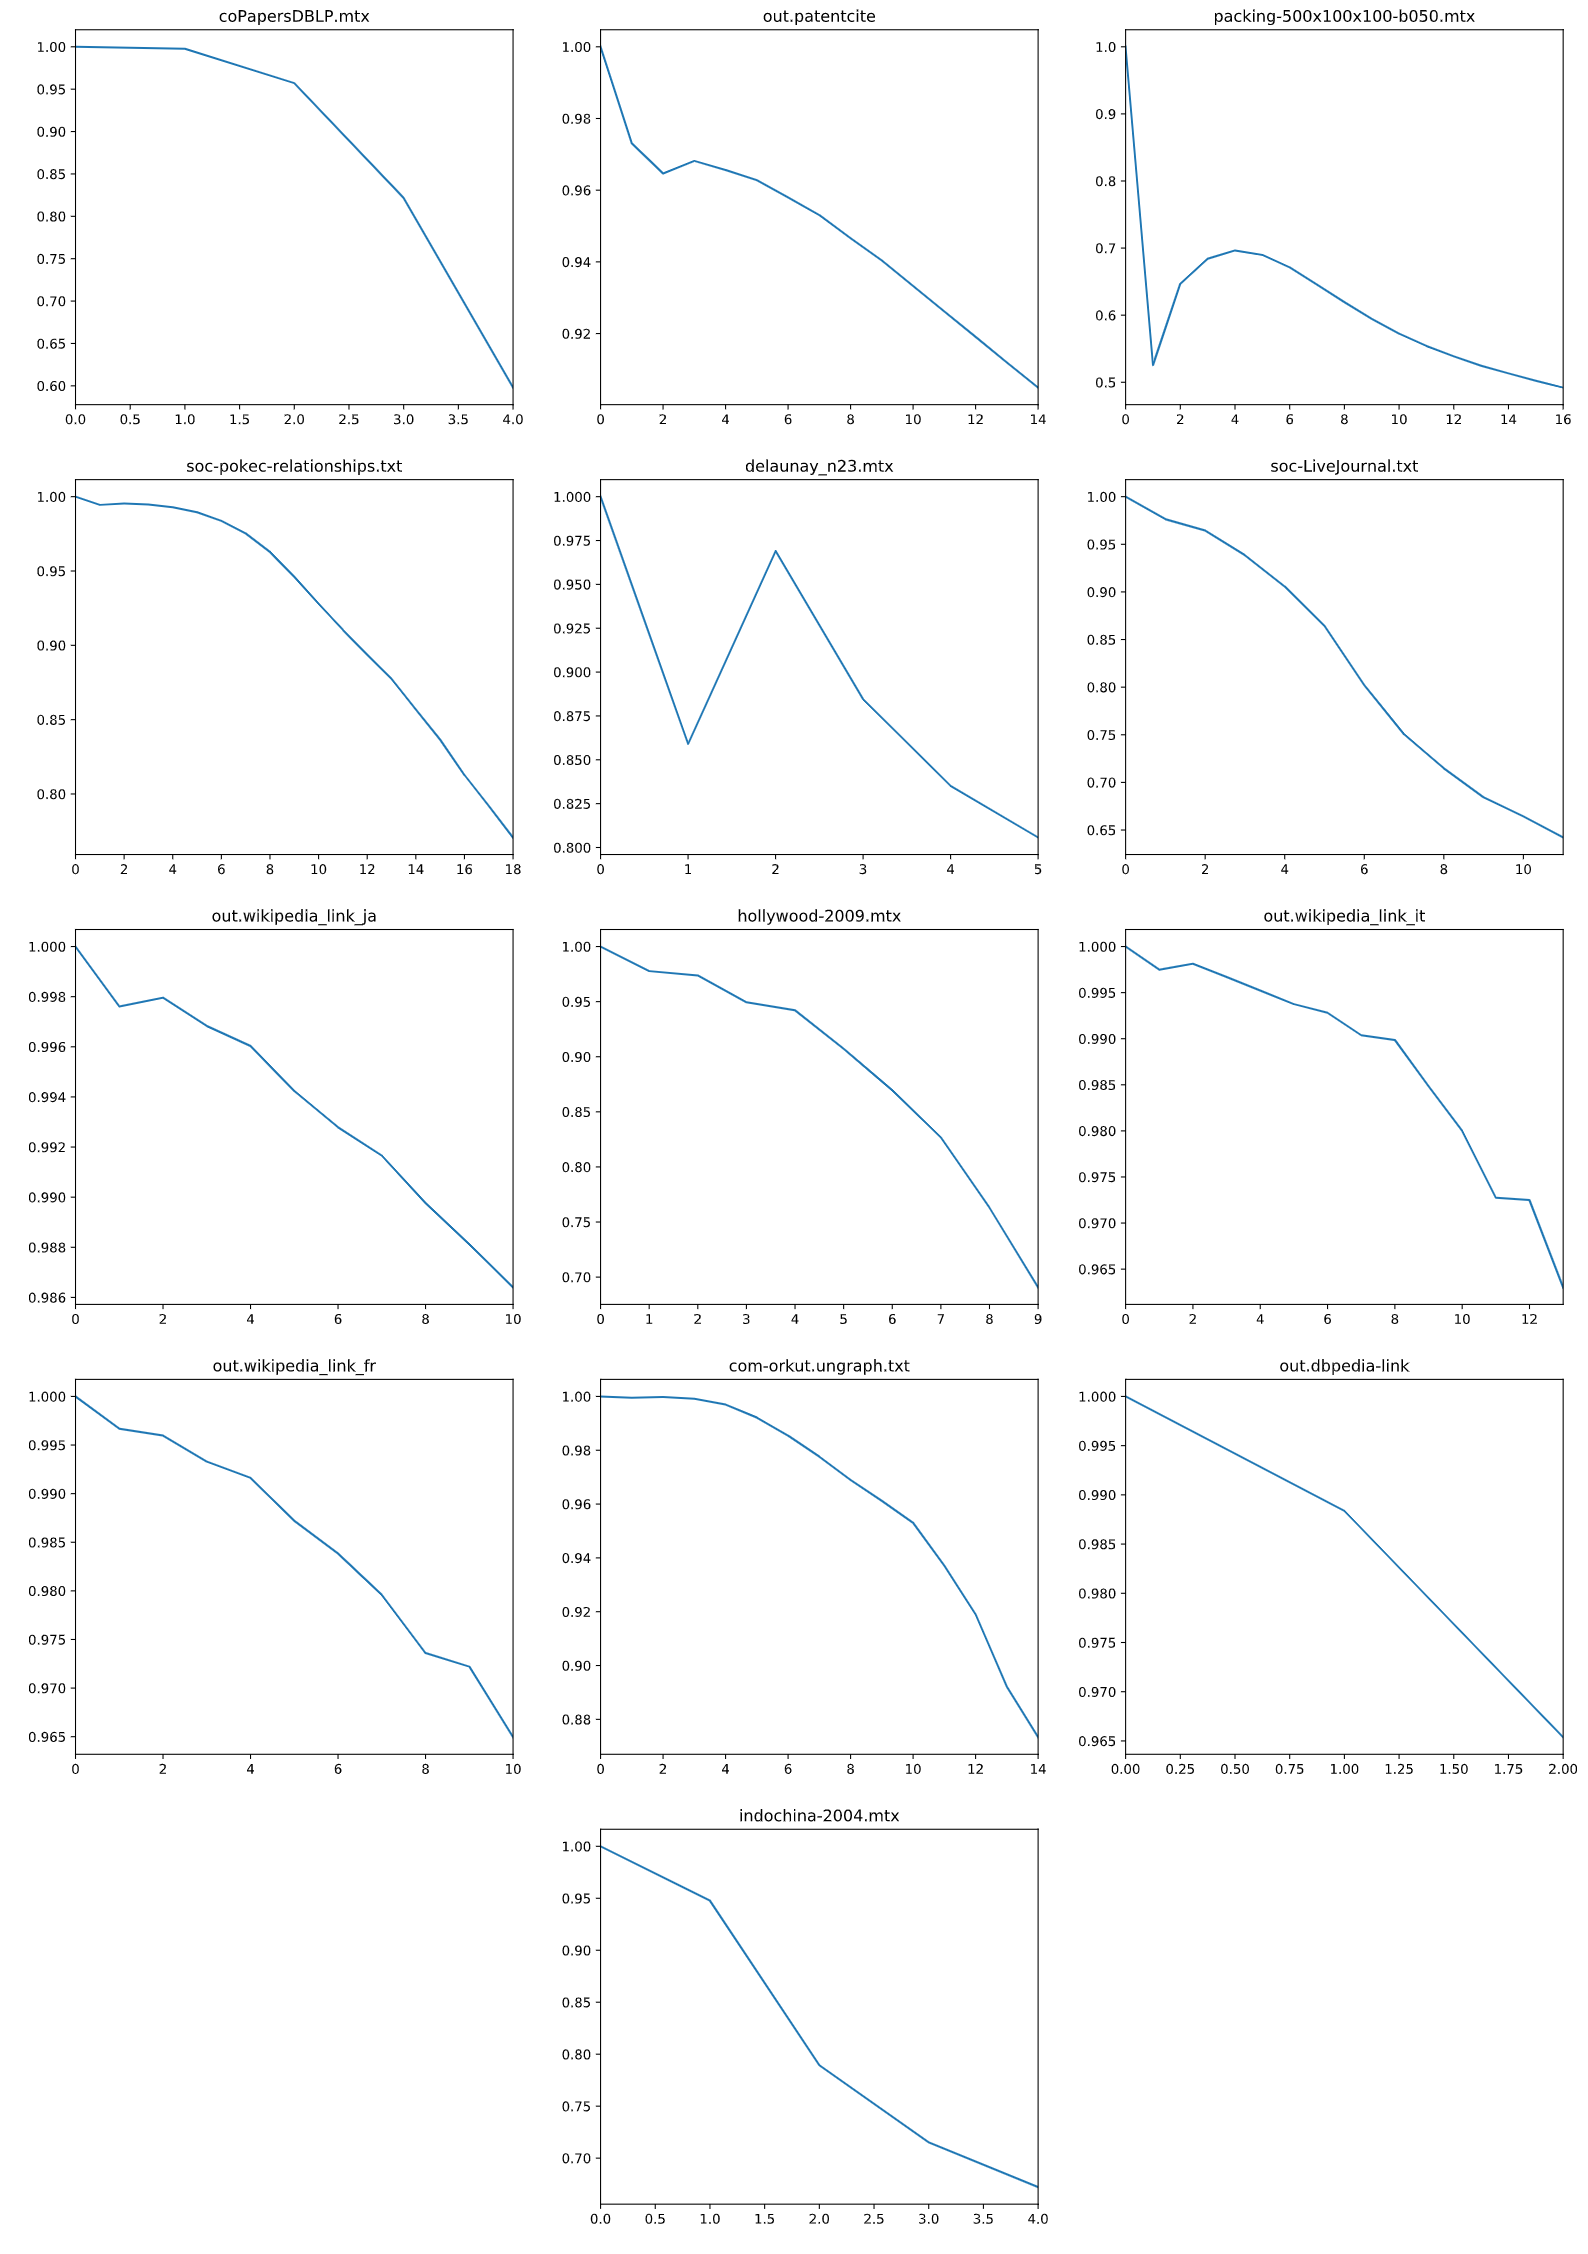
\includegraphics[width=0.7\linewidth]{0-resources/edge-percentage}
	\caption{CAMBIARE IMMAGINE}
	\label{fig:prun-vs-no}
\end{figure}
Now we evaluate the impact in terms of time of the pruning approach in the Prune-Sort-Reduce algorithm: to do this, we create a comparison version of the algorithm from the presented one. This version doesn't prune the node in the Copy sub-phase and doesn't collect the data used to create the support pruning array in the last two sub-phases (the first one only update the community assign to each node; the second one is skipped). The results are illustrated in the Figure \ref{fig:prun-vs-no}. We exclude from this graphic the first iteration because this one doesn't make the same step of the other due to its special optimization (Chapter \ref{f-1}). We notice that the reduction in terms of times in the pruning version is proportional to the reduction of edges analyzed. 
\begin{figure}[h]
	\centering
	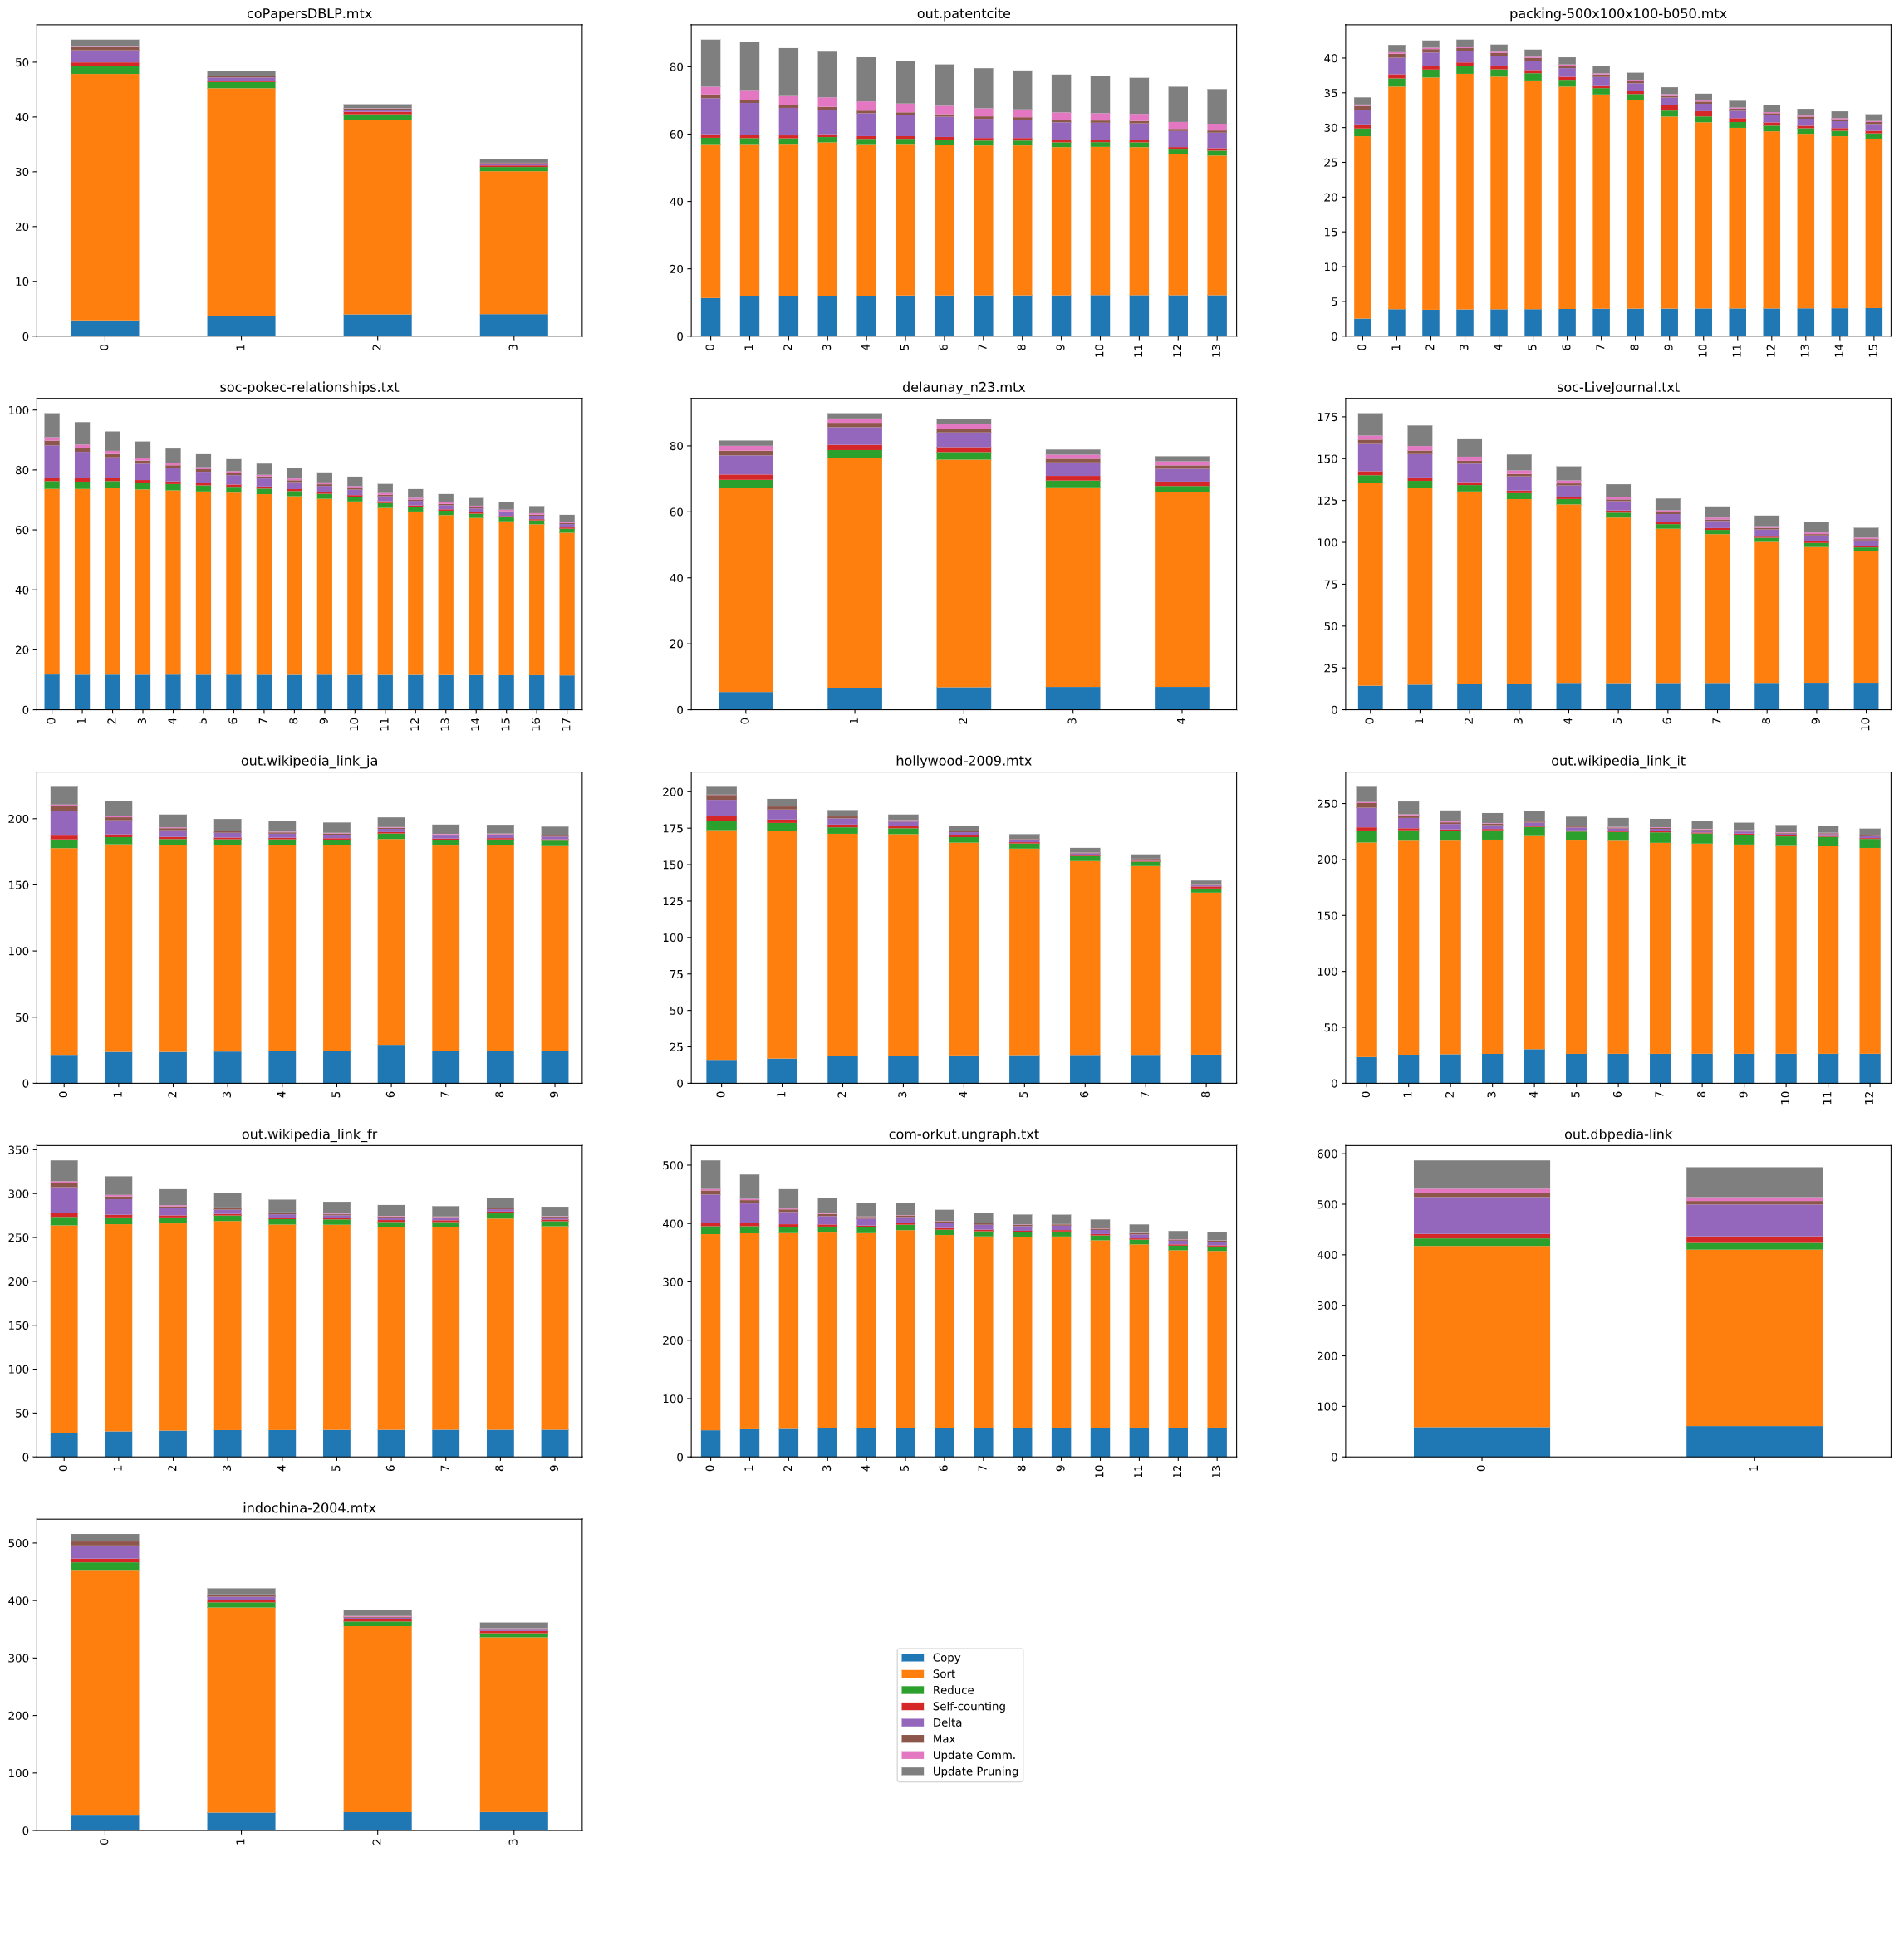
\includegraphics[width=1\linewidth]{0-resources/suphases-sort.png}
	\caption{}
	\label{fig:suphases-sort}
\end{figure}
In the Figure \ref{fig:suphases-sort} is illustrated the contribution of each sub-phase in terms of time to the total one for each iteration.
As expected, the Sort sub-phase is the most consuming one: indeed this sub-phase at least 50\% of the time, reaching even more than 80\% of the time in the first and in the last graph. We notice also that the pruning on the data in input have a direct effect on the sorting phase and the greatest gain in terms of time become from the optimization of this sub-phase. 


\subsection{Algorithms comparison}
In this section, we focus our analysis on the comparison between the two algorithm in order to find advantages and disadvantages of each method. 
First of all, we notice from the Table \ref{tab:mod} that the two algorithm obtain a very similar score of modularity. In the Figure \ref{fig:modularity-progression}, we expose the progression of the modularity $Q$ in the first operation. As we can see, the modularity in the two algorithms grows in almost identical way: this is due to the minimum labelling heuristic (Chapter \ref{parallel-imp}) that force the algorithms to converge to a similar result. 
\begin{figure}[h]
	\centering
	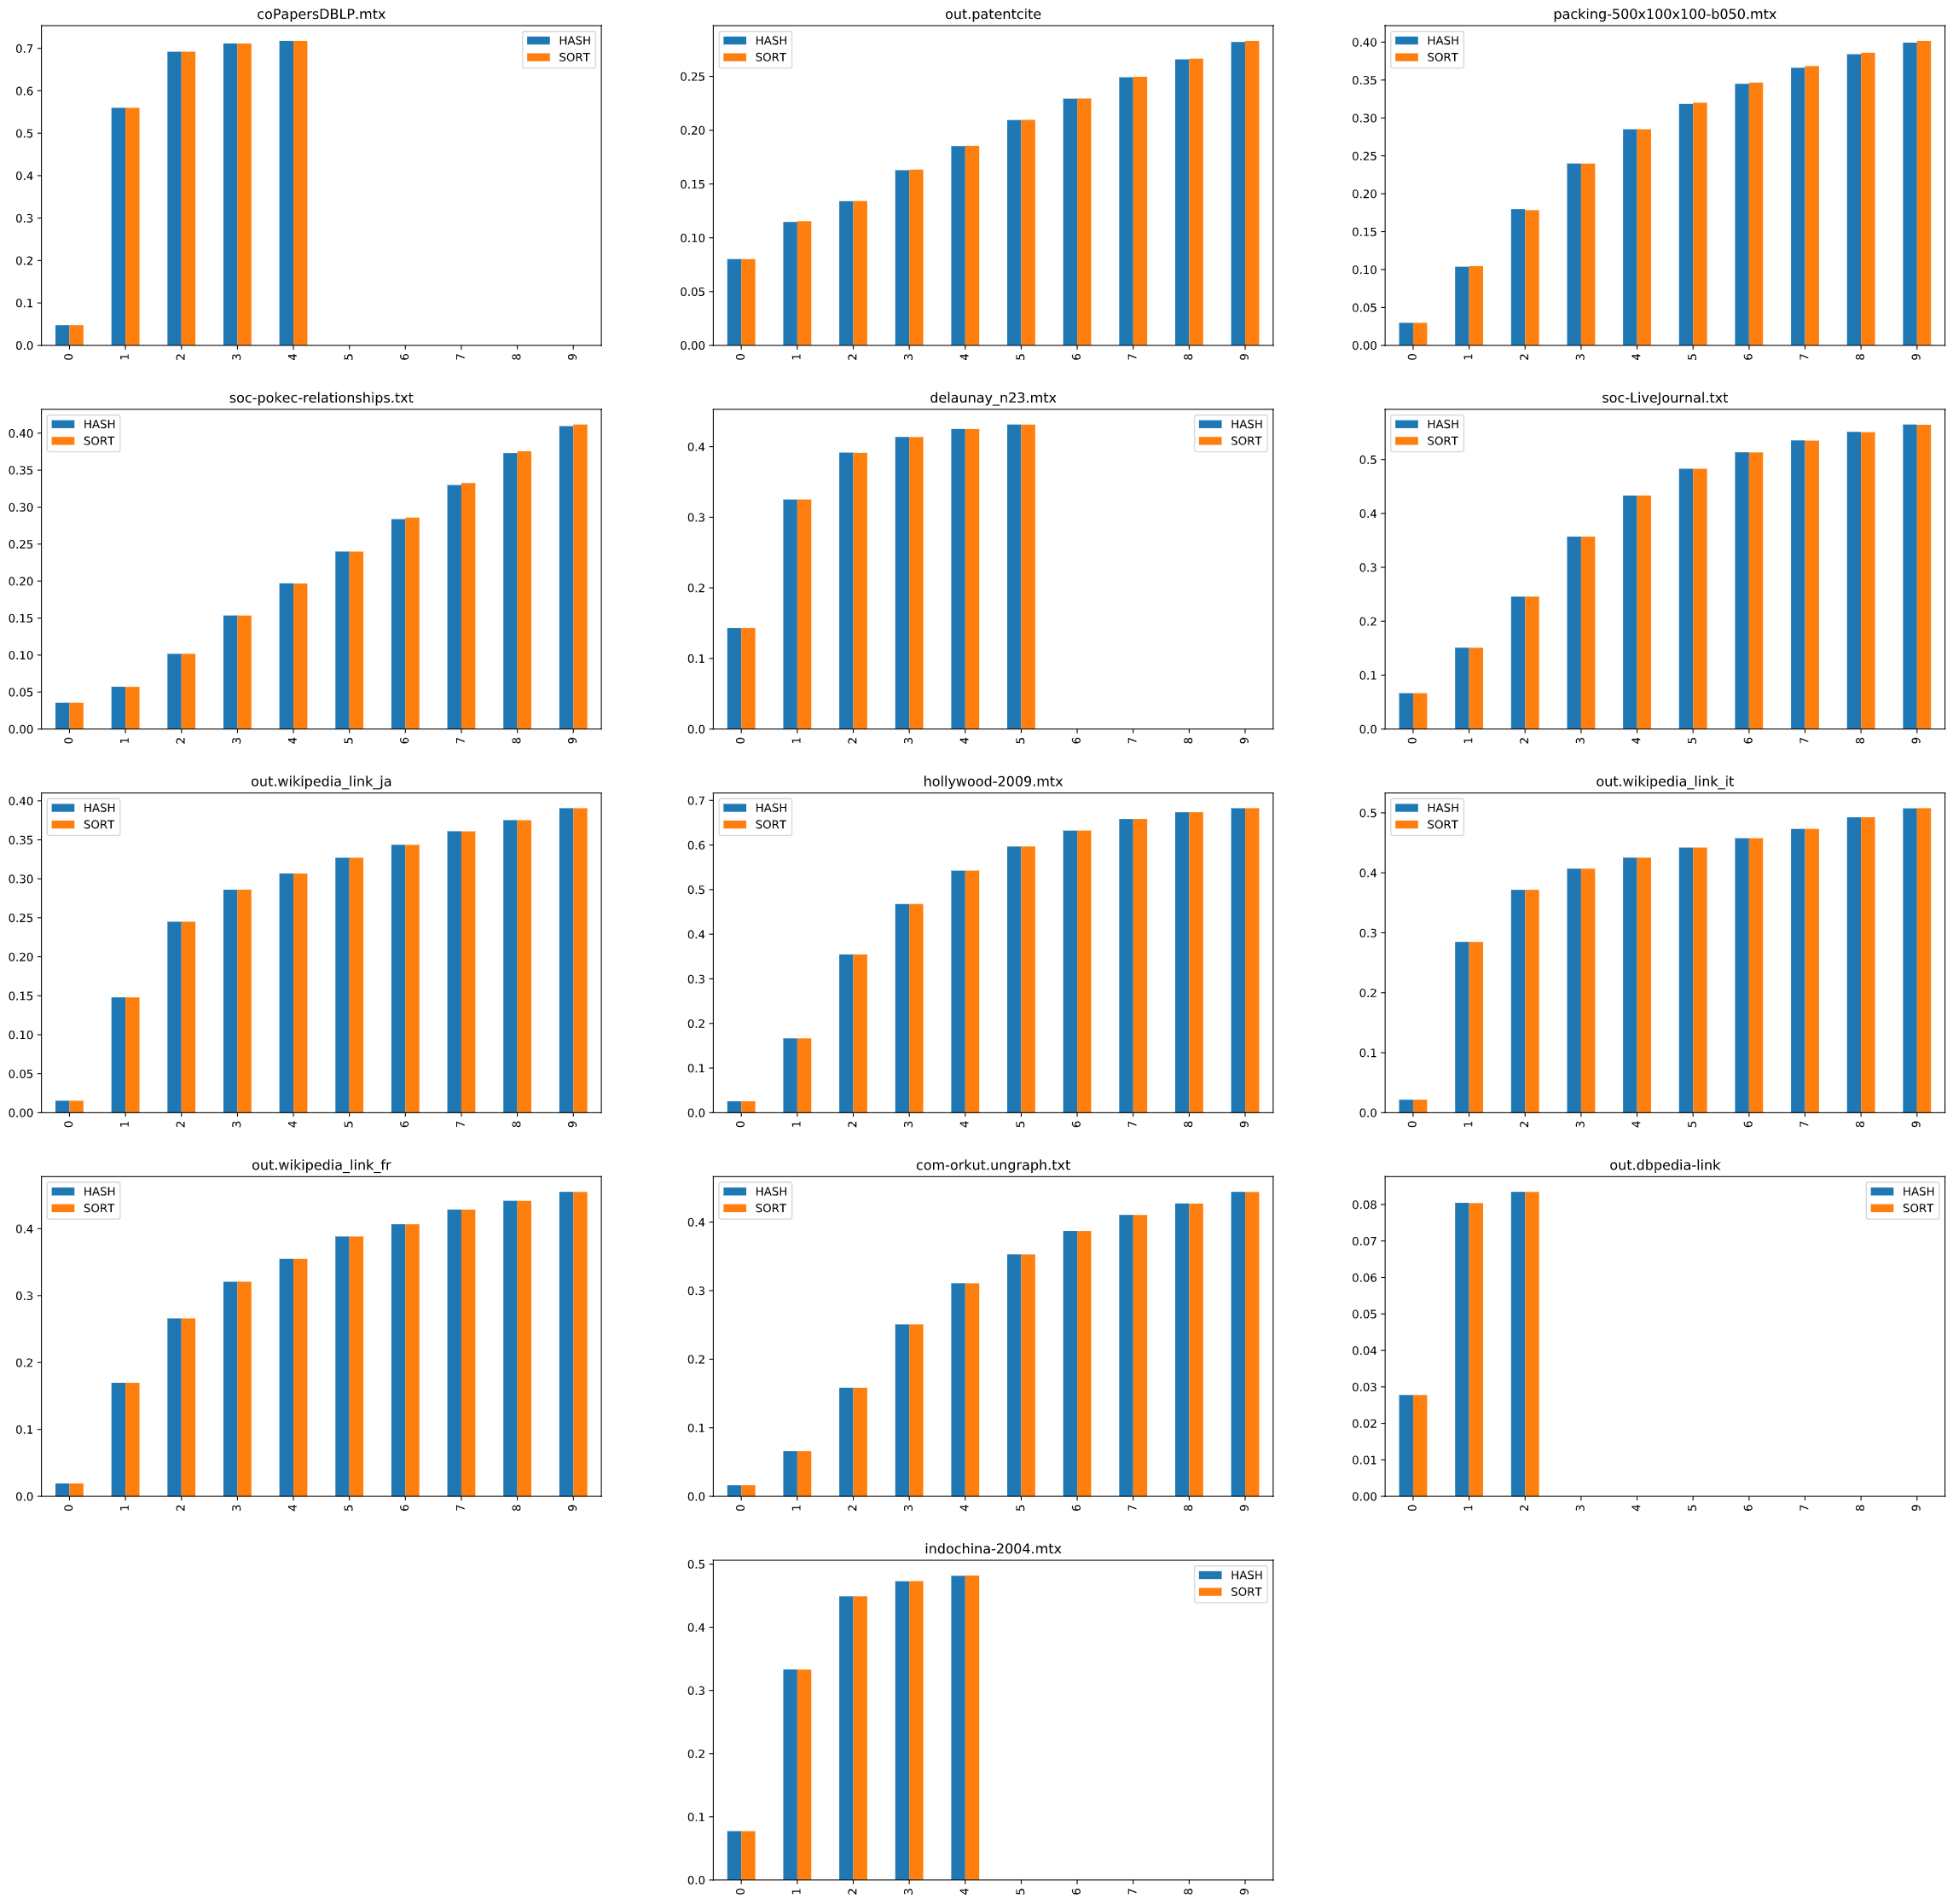
\includegraphics[width=1\linewidth]{0-resources/modularity-progression}
	\caption{Modularity Progression in the first iteration}
	\label{fig:modularity-progression}
\end{figure} 

First of all, we compare the iterations of the first optimization phase in terms of times ()
\begin{figure}[h]
	\centering
	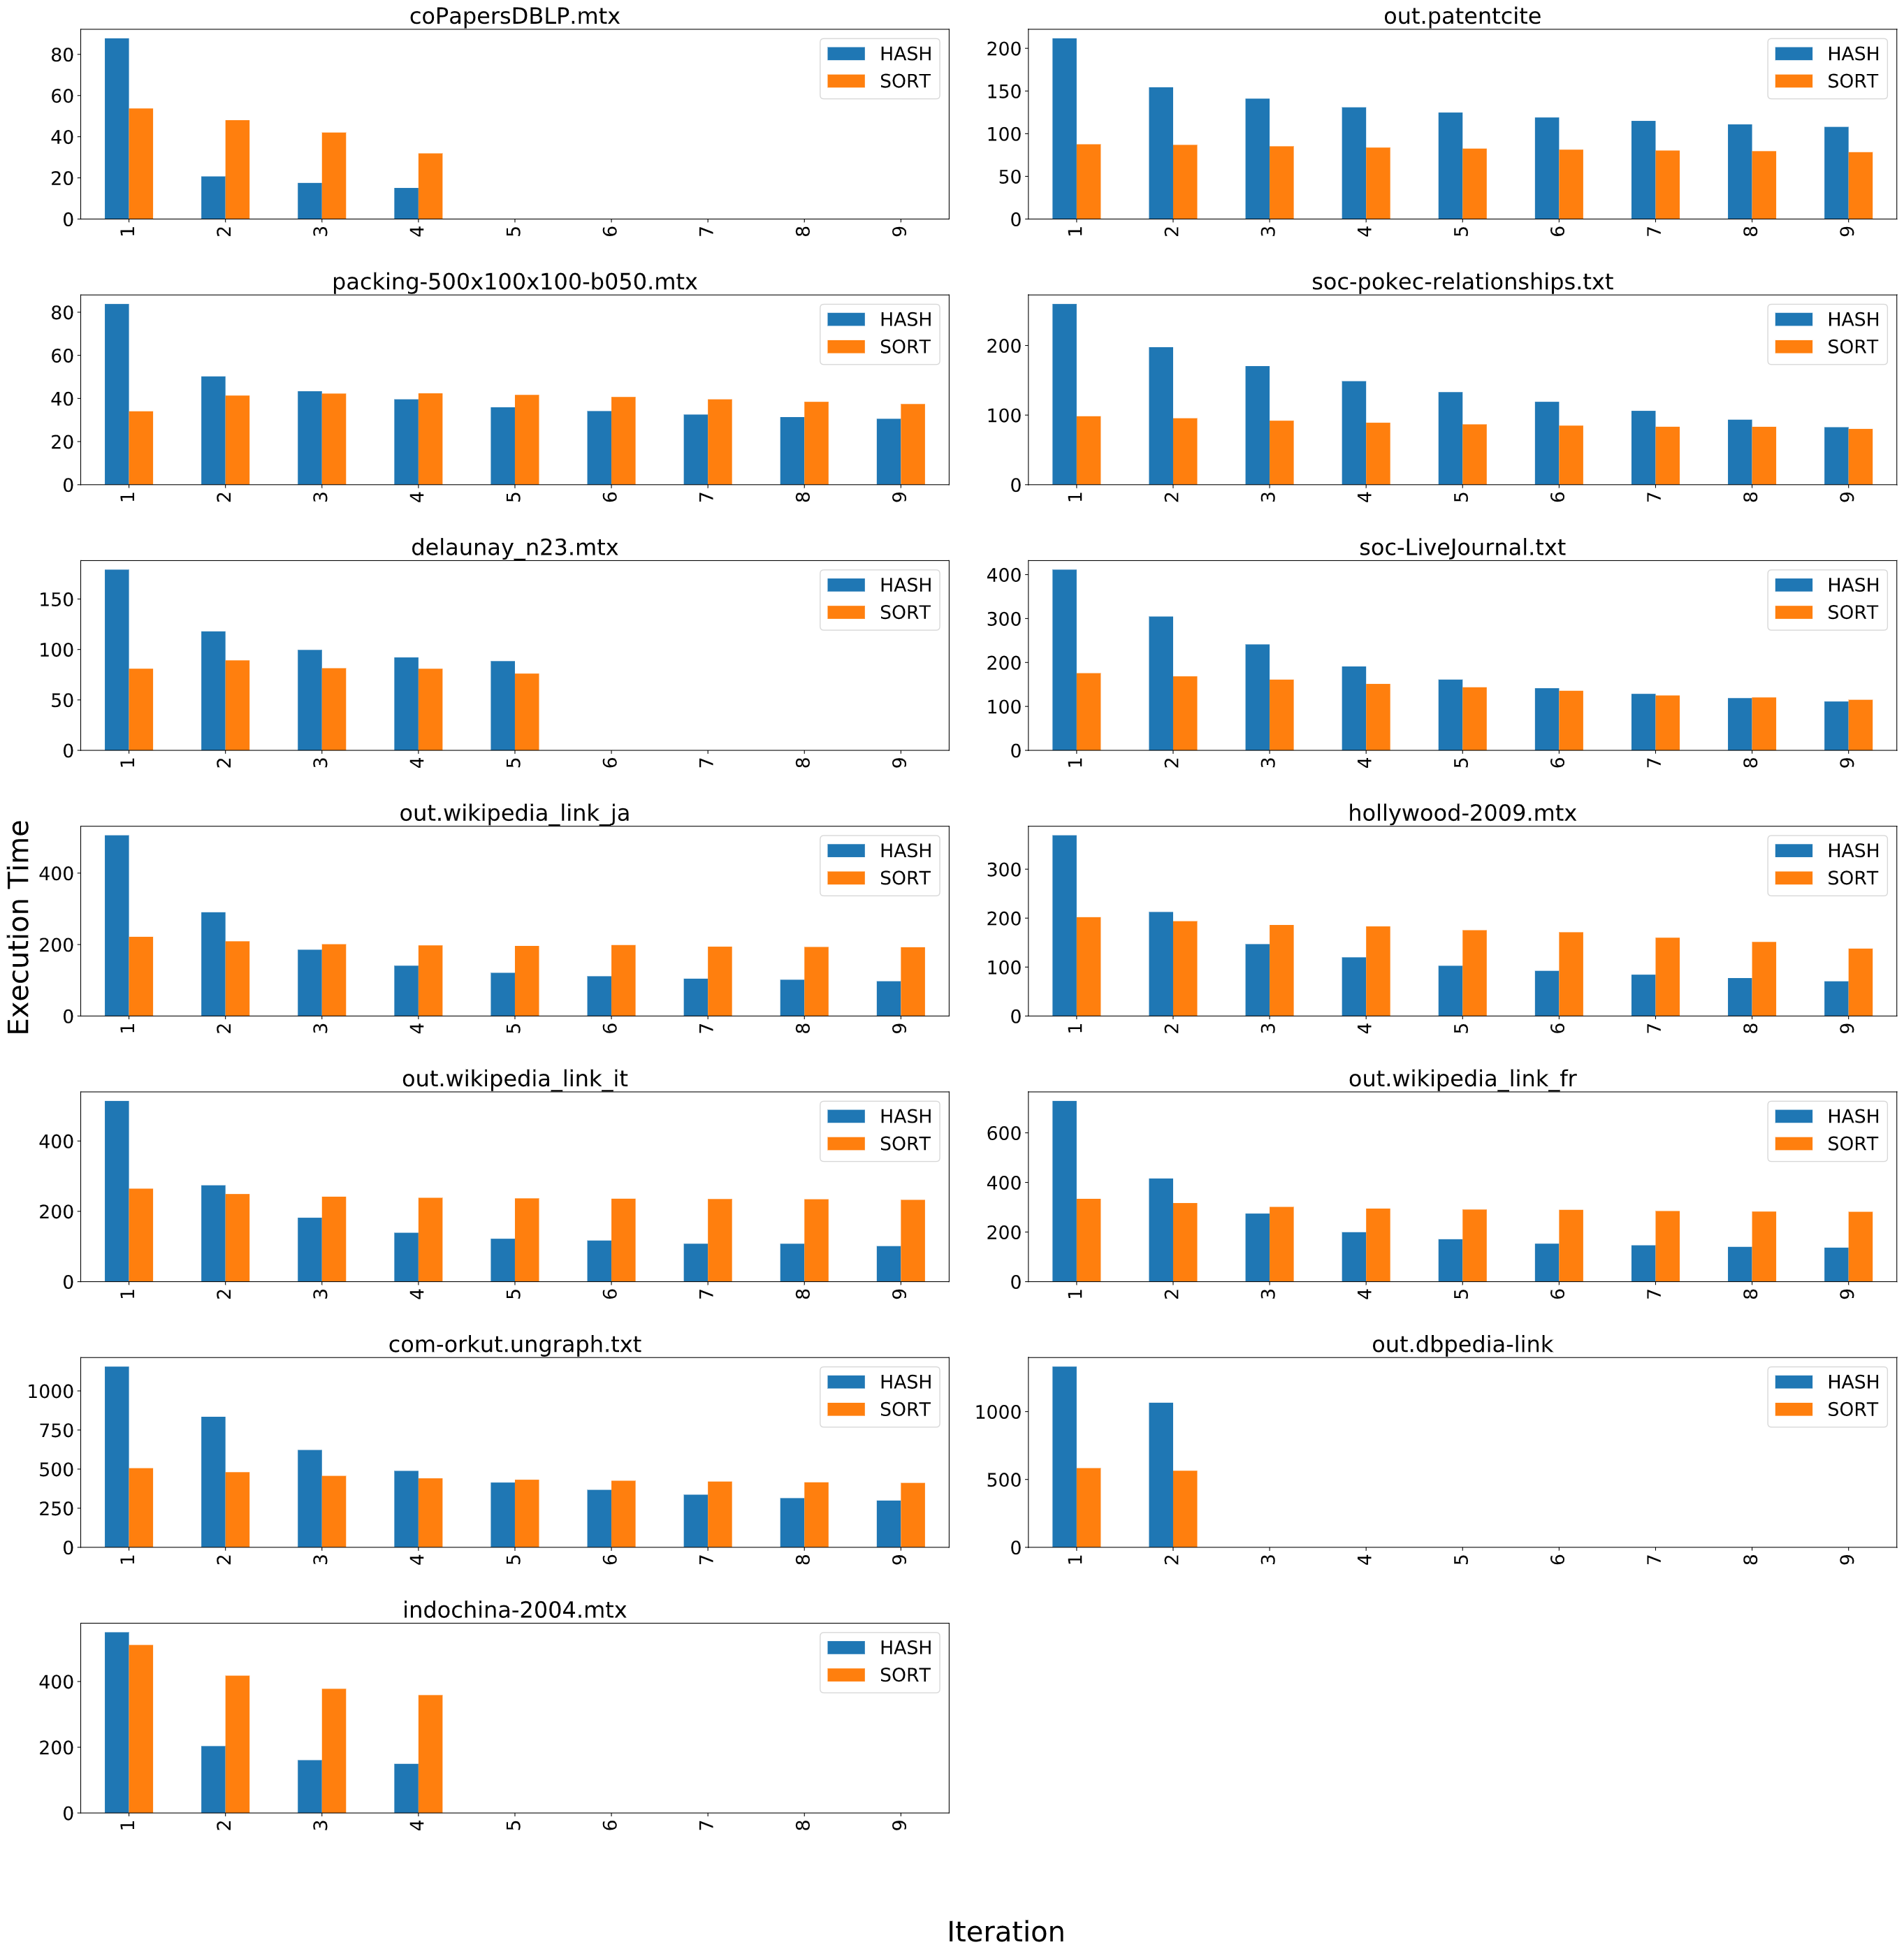
\includegraphics[width=1\linewidth]{0-resources/hash-vs-sort}
	\caption{Time of the first ten iteration of the first optimization phase.}
	\label{fig:hash-vs-sort}
\end{figure}



